\documentclass[times, utf8, seminar, numeric]{fer}
\usepackage{booktabs}
\graphicspath{ {./slike/} }

\begin{document}

\title{Aplikacija za pomoć pri učenju sviranja klavira}

\author{Ana Bagić}

\voditelj{Marko Čupić}

\maketitle

\tableofcontents

\chapter{Uvod}
Danas je učenje sviranja raznih instrumenata puno dostupnije nego prije široke primjene Interneta. Veliku ulogu u tome imale su video streaming platforme, posebice YouTube, gdje je dostupno jako puno besplatnih video-materijala koji na razne načine pomažu zainteresiranima u svladavanju sviranja instrumenata po želji. Osim videozapisa, vrlo su popularne i aplikacije koje kroz kraće lekcije uče korisnike sve od osnova poput ljestvica, do zahtjevnijih pjesama. Daleko najpopularniji instrument na tim platformama je klavir.\\

U okviru završnog rada napravila sam aplikaciju koja na temelju videozapisa generira notni zapis. U videozapisu se okomitim padajućim linijama prikazuju note koje se trebaju svirati u tom vremenskom intervalu. Analizom slika (engl. \textit{frames}) iz videozapisa određivala sam pozicije i duljine tih linija i na temelju njih gradila notni zapis. Za bilježenje notnog zapisa koristila sam MusicXML\cite{musicxml} format koji je široko korišten i kojega podržava većina aplikacija za uređivanje, stvaranje ili reproduciranje glazbe.\\

U ovome radu postaviti ću smjernice za buduću izradu projekta i diplomskog rada. U dogovoru s mentorom, odlučila sam da ću u diplomskom radu poboljšati i nadograditi svoj završni rad. Kroz ovaj seminar, istražiti ću moguće nadogradnje postojećeg programskog rješenja završnog rada, te izraditi nove funkcionalnosti u obliku aplikacije za pomoć pri učenju sviranja klavira uz praćenje korisnika. Za razliku od većine postojećih, ovo će biti besplatna aplikacija otvorenog koda (engl. \textit{open-source}). Zbog nekih mogućnosti koje nudi operacijski sustav Linux, za početak ću implementaciju raditi za njega, te kasnije proširiti na Windows i MacOS ako budem mogla.

\chapter{Opis problema}
Kroz ovaj seminar istražiti ću dva problema. Prvi će biti kako mogu poboljšati implementaciju generiranja notnog zapisa na temelju videozapisa sviranja klavira koju sam napravila u okviru završnog rada. Proučiti ću mogu li koristiti neke drugačije tehnologije i pristupe nego što sam do sada koristila kako bih povećala točnost i brzinu algoritma. Drugi problem biti će kako napraviti aplikaciju koja se preko računala može povezati na klavijaturu i u stvarnom vremenu pratiti sviranje korisnika. Aplikacija će moći prikazivati korisniku što treba svirati i dati mu povratnu informaciju o njegovom uspjehu. Ova dva dijela spojiti će se u jednu aplikaciju kako bi korisnik mogao unijeti videozapis s pjesmom koju želi naučiti svirati, te zatim dobiti notni zapis pjesme i mogućnost učenja sviranja kroz aplikaciju.

\section{Generiranje notnog zapisa na temelju videozapisa}
Format (izgled) videozapisa koji se može koristiti za generiranje notnog zapisa prikazan je na slici \ref{fig:nttdscreen}. Plavi i zeleni pravokutnici predstavljaju tipke klavijature koje se trebaju stisnuti kada pripadajući pravokutnici dođu u doticaj sa klavijaturom. U ovom primjeru plavi pravokutnici predstavljaju note svirane lijevom rukom, a zeleni desnom.

\begin{figure}[h]
	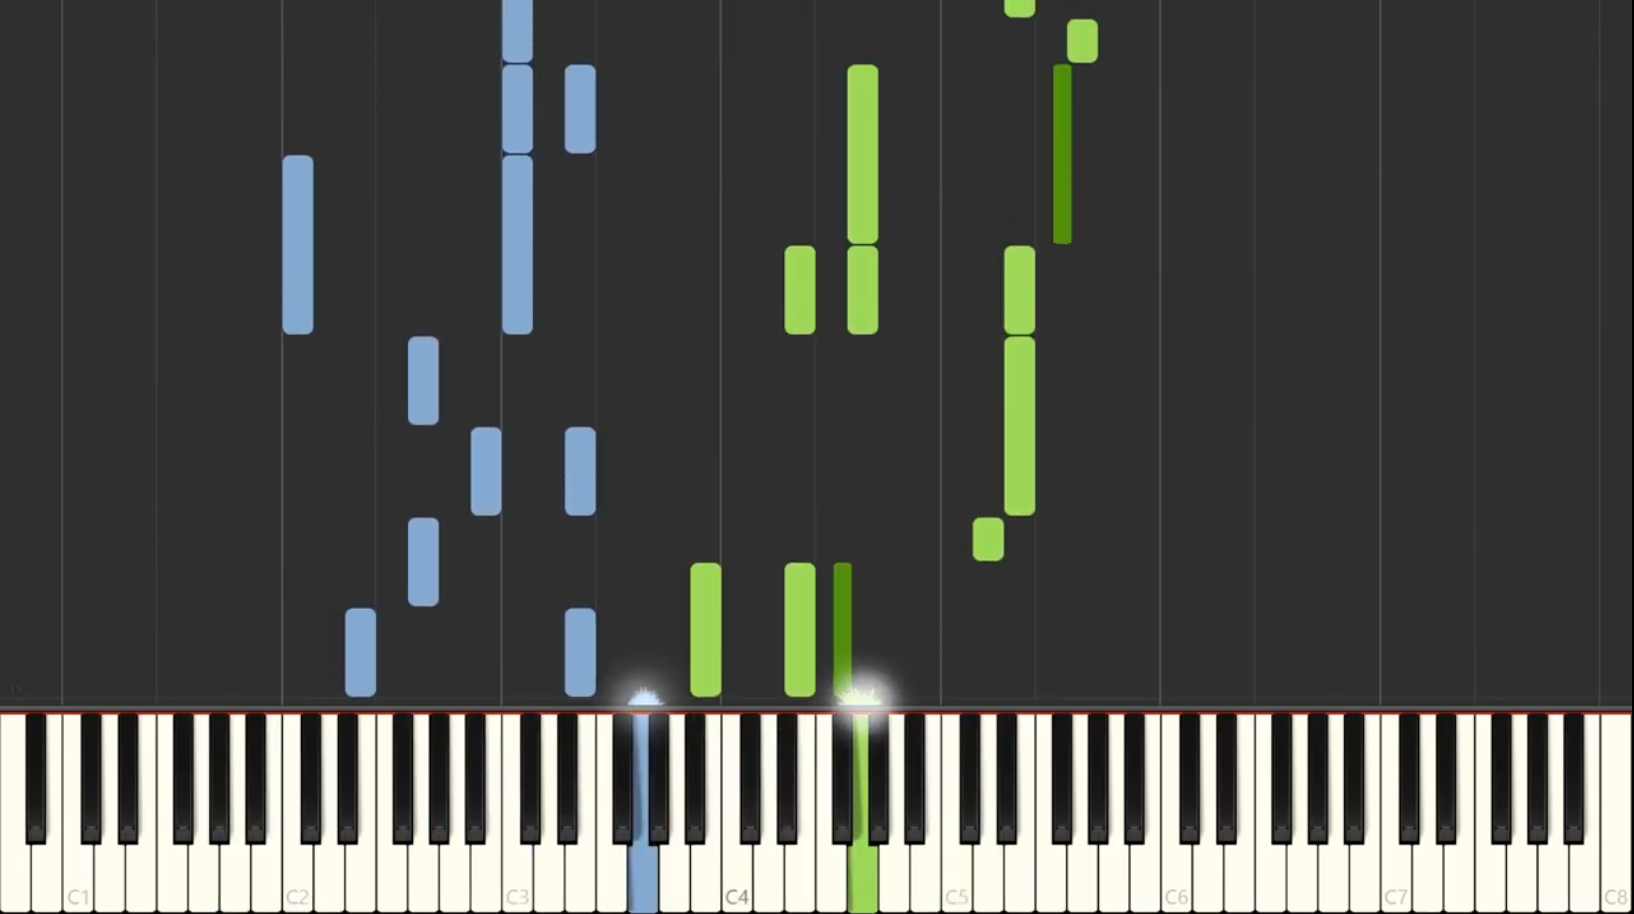
\includegraphics[scale=0.24]{nttdscreen.png}
	\centering
	\caption{Snimka zaslona korištenog videozapisa\cite{nttd}}
	\label{fig:nttdscreen}
\end{figure}

Iako moja trenutna implementacija radi relativno dobro, ima puno prostora za napredak. Ona nije dovoljno robusna za različite rubne slučajeve. Smanjivanjem kvalitete videozapisa, naravno smanjuje se i točnost generiranog notnog zapisa. Osim same kvalitete, na točnost utječe i "šum" u videozapisu: efekti (npr. iskrice koje se mogu vidjeti na slici \ref{fig:nttdscreen}) koje autori videozapisa dodaju kako bi ga učinili zanimljivijim gledateljima.\\

Uz točnost, jedna od glavnih stvari koje bih htjela poboljšati u novoj implementaciji je brzina izvedbe. Trenutno, za pjesmu od oko 3 minute treba skoro toliko dugo da se generira notni zapis. Razlog tome je što sam svaku sliku (engl. \textit{frame}) videozapisa obrađivala i iz nje izvlačila podatke o trenutnoj poziciji svih pravokutnika. Iako je to jako mali dio koda u odnosu na cijeli projekt, zahtjeva daleko najviše vremena za izvođenje. Iz tog razloga mislim da nema puno prostora gdje bi ikakva optimizacija pomogla, nego bi trebalo na drugačiji način pristupiti rješavanju tog problema.\\

Idući problem koji bih trebala riješiti je određivanja raspona klavijature, mjere i tempa pjesme iz videozapisa. To su sve informacije koje u trenutnoj implementaciji korisnik treba sam unijeti, kao što se može vidjeti na slici \ref{fig:screen2}. Za određivanje raspona klavijature sam već imala neke ideje, međutim zbog jednostavnosti sam ipak odlučila da korisnik to unese sam. Određivanje mjere pjesme i tempa je vrlo vjerojatno najteži problem ovoga rada (možda čak i nemoguć zbog višeznačnosti).

\begin{figure}[h]
	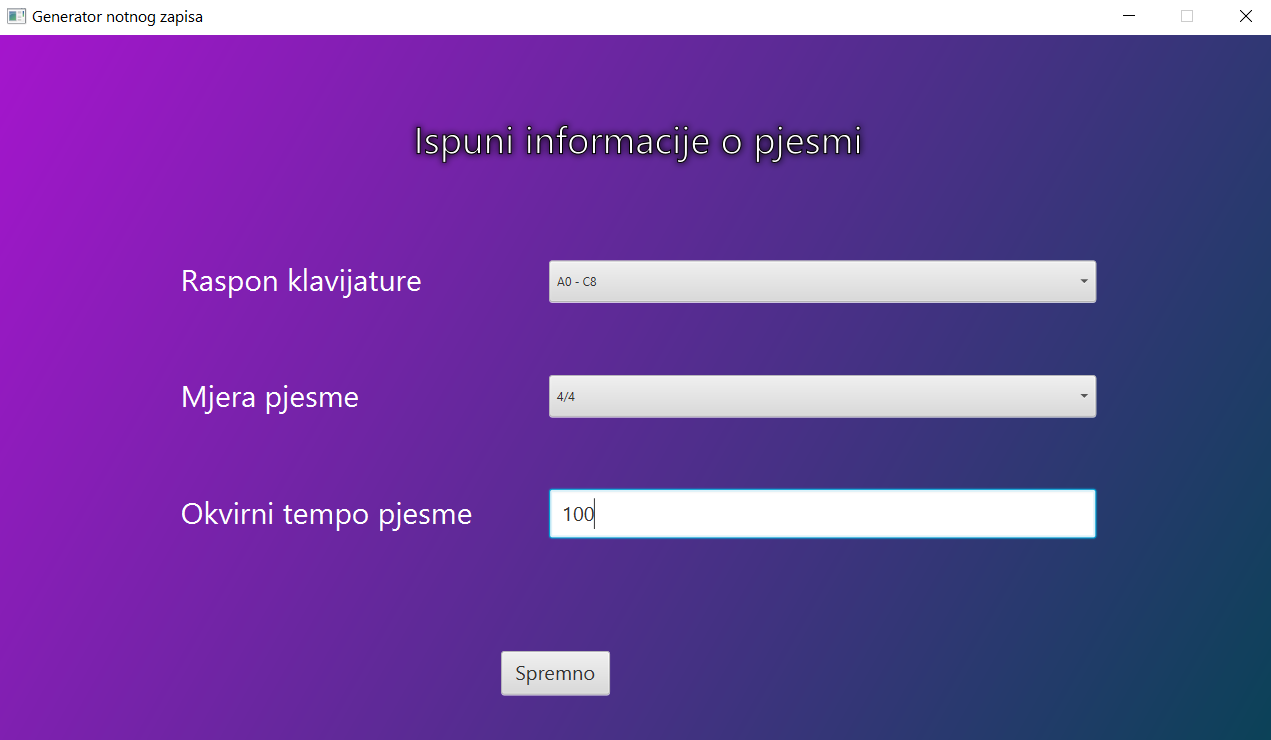
\includegraphics[scale=0.43]{screen2.png}
	\centering
	\caption{Snimka zaslona za određivanje parametara pjesme}
	\label{fig:screen2}
\end{figure}

Jedan od problema koji nije toliko veliki i već u trenutnoj implementaciji funkcionira dosta dobro je određivanje tonaliteta pjesme. Trenutna implementacija se zasniva na brojanju pojavljivanja svih tonova u cijeloj pjesmi, te određivanje tonaliteta na temelju zastupljenosti tonova koji čine tonički akord (prvi, treći i peti stupanj ljestvice). Takav pristup je dovoljno dobar većinu vremena, jer većina pjesama poštuje taj zakon. Međutim, nekada bi dobro bilo uzeti u obzir pojavljivanje svih tonova tonaliteta, a to onda dovodi do puno uvjetnog grananja u kodu (što nikada nije dobra praksa) i velikog broja rubnih slučajeva koje bi trebalo obraditi.\\

Zadnja stvar koju bih htjela izmjeniti u postojećem rješenju je dobivanje notnog zapisa. Trenutno, aplikacija kao izlaz "izbaci" dokument u MusicXML formatu. Osobi koja želi dobiti čitljivi notni zapis, to ništa ne znači. Ona treba pomoću neke druge aplikacije iz MusicXML formata dobiti PDF datoteku ili pregledavati notni zapis u korisničkom sučelju (npr. Noteflight\footnote{noteflight.com}, MuseScore\footnote{musescore.com}, Soundslice\footnote{soundslice.com}). Htjela bih izbjeći taj međukorak, te korisniku ponuditi punu funkcionalnost u mojoj aplikaciji.\\

Ovo su glavni problemi koje bih htjela rješiti. Nisam sigurna hoću li moći riješiti sve od njih, a možda i tijekom implementacije naiđem na još neki, no smatram da je ovo dobar početak.

\section{Praćenje sviranja korisnika}
Drugi problem koji ću riješiti je na koji način mogu putem aplikacije pratiti sviranje korisnika. Istražiti ću način spajanja klavijature (engl. \textit{synthesizer}), odnosno električnog klavira na računalo. Na koji način se prenose informacije o sviranim tonovima, te kako ih mogu obraditi i prikazati korisniku njegov napredak.\\

Ideja aplikacije je da korisnik unese pjesmu koju želi naučiti svirati u nekom formatu koji podržava računalo (vrlo vjerojatno će to biti MusicXML i/ili MIDI\footnote{en.wikipedia.org/wiki/MIDI}). Aplikacija će prikazivati korisniku note koje treba svirati i pratiti njegov uspjeh. Podržavati će dva načina rada: lakša i teža verzija. Kod lakše verzije aplikacija će čekati dok korisnik ne stisne ispravnu notu. U težoj verziji, aplikacija će u tempu pjesme prikazivati note, kako bi se pomoglo korisniku da izvježba pjesmu u pravom tempu. Nakon završetka pjesme, korisnik će dobiti povratnu informaciju o uspjehu (npr. postotak točno odsviranih nota, držanje tempa, ...).\\

Korisnik će moći odabrati želi li vježbati samo jednu ruku (posebno lijevu ili posebno desnu) ili obje u isto vrijeme. Ova funkcionalnost je dosta bitna za glazbenike, jer većina klavirista odvojeno vježba svaku ruku, pošto to dosta olakšava učenje.
 
\chapter{Prijedlog implementacije}
U nastavku ću iznijeti moju ideju implementacije prethodno navedenih problema. Iako mi sada ta rješenja zvuče dobro, tek kada krenem sa implementacijom ću saznati jesu li izvediva i hoće li funkcionirati kako sam zamislila.

\section{Generiranje notnog zapisa na temelju videozapisa}
Prvi problem koji bih htjela riješiti je brzina izvođenja programa. Prva ideja koja mi je pala na pamet je paralelizacija programa, odnosno primjena višedretvenosti. Međutim, tu bi bilo veoma teško odrediti granicu između zadataka, pošto je teško grupirati note u određeni takt ako zadatak nema informaciju o prethodnim notama. Iako ovo rješenje zvuči dosta komplicirano, možda nije nemoguće ali definitivno trebam tome posvetiti još vremena kako bih smislila i isprobala neke ideje razdvajanja.\\

S druge strane, praćenje objekata (engl. \textit{object tracking}\cite{tracking1}) mi se čini kao rješenje koje osim što je učinkovitije, također je i preciznije. Do sada sam u radu koristila samo praćenje objekata (engl. \textit{object detection}\cite{tracking2}), koje je u slici pronalazilo konture objekata, a pomoću njih i granični okvir (engl. \textit{bounding box}). To sam radila za svaku sliku videozapisa, te pomoću svojeg algoritma pratila identitet pravokutnika. Međutim, već postoje algoritmi praćenja objekata u videozapisu koji su sigurno efikasniji i točniji od moje implementacije\cite{tracking3}.\\

Praćenje objekata u videozapisu kombinira detekciju objekata u statičkim slikama i informacije iz videozapisa kako bi se predvidjele putanje kretanja tih objekata. Kod praćenja više objekata, treba se prvo identificirati svaki objekt, te zatim pratiti njegovo kretanje kroz vrijeme dok ne napusti okvir. Najčešći problemi ovim algoritmima su prekrivanje jednog objekta drugim (što meni ne bi trebalo stvarati probleme jer je svaki pravokutnik na svojem dijelu slike) i stapanje objekta s pozadinom (također mi ne bi trebao biti problem zbog očitih granica između traženih pravokutnika i pozadine).\\

Kad sam tek krenula s implementacijom završnog rada, imala sam ideju da raspon klavijature odredim "brojajući" tipke prikazane klavijature sa dna videozapisa. Međutim, vrlo brzo sam shvatila da to nije idealno rješenje jer mi broj tipki ne daje do znanja koje "područje" klavijature je zahvaćeno videozapisom. Većina videozapisa obuhvaća klavijaturu klasičnog koncertnog klavira, odnosno 88 tipki (7 i pol oktava), no nije uvijek tako. Neki od videozapisa, pogotovo oni namijenjeni početnicima, prikazuju samo dio pune klavijature, najčešće 3 do 5 oktava. Iz tog razloga, čak i znajući koliko tipki sadrži klavijatura, treba odrediti koji je to raspon. Pozicijom crnih tipki moglo bi se utvrditi s kojom tipkom (tonom) počinje, međutim veliki problem je određivanje oktave. U većini videozapisa na \textit{c} tipki piše u koju oktavu spada, ali to najčešće bude toliko slabo napisano, da i ljudsko oko jedva prepozna. Mogla bih pretpostaviti da će uvijek nota \textit{c3} biti blizu centra klavijature, pošto je takva situacija u većini pjesama, ali to ne bi bilo ispravno za sve pjesme. Zbog toga, točan raspon klavijature neće biti moguće skroz ispravno odrediti pošto algoritam ne uzima zvuk u obzir.\\

Kao što sam već navela prije, određivanje tempa i mjere pjesme je vjerojatno najizazovniji zadatak ovog rada. Problem je što je tempo, u nekom slučaju, subjektivan pojam, u smislu da iako bi bilo jednostavno razlikovati između tročetvrtinske i četveročetvrtinske mjere, teško je odrediti koja pjesma pripada četveročetvrtinskoj, a koja četveroosminskoj. Bez notnog zapisa, smatram da nije moguće uvijek potpuno točno odrediti, jer uvijek postoji mogućnost da je pjesma u sporoj četveročetvrtinskoj mjeri ili brzoj četveroosminskoj. Za ovaj problem mi još nije sinulo rješenje, tako da ću to još istraživati do diplomskog rada. U planu mi je popričati sa nekim ljudima koji se profesionalno bave glazbom (pogotovo klaviristima) kako bih, nadam se, dobila neki savjet za pristup tom problemu.\\

Mislim da bi se tonalitet pjesme mogao dosta efikasno i točno odrediti koristeći logističku regresiju. Kao ulaz u model postavila bih broj pojavljivanja određenog tona kroz pjesmu, a izlazi bi mi bili tonaliteti. Znači dimenzija ulaza bila bi 12 (7 bijelih tipki/tonova i 5 crnih), a izlaza 24 (12 durskih i 12 molskih tonaliteta). Eventualno se na ulaz može dodati još jedna značajka koja označava s kojim tonom je završila skladba/pjesma. Smatram da bi uz te značajke model bio dosta precizan. Ovaj model bi vjerojatno bio puno robusniji od moje prve implementacije za maleni ulaz (npr. kada postoji mali broj nota). Zbog toga bih ovim pristupom mogla riješiti problem kada se tonalitet mijenja unutar pjesme. Svaka mala grupa taktova (možda 2 do 4 takta odjednom) bi se mogla zasebno obrađivati, te bi model mogao dati predikciju za svaku takvu grupu posebno. Trebalo bi eksperimentalno odrediti veličinu te grupe, međutim pretpostavljam da je najpametnije da ona bude višekratnik broja 2, pošto je glazba najčešće građena s takvim blokovima.\\

Zadnji problem koji bih htjela rješiti je integracija konverzije MusicXML u PDF format. Sama u sklopu diplomskog rada ne mogu ovo napraviti jer je prekomplicirano i previše vremena bi mi uzelo, ali na sreću postoje već gotovi besplatni alati na Internetu koji mi mogu pomoći s ovime. Aplikacija MuseScore ima svoju besplatnu aplikaciju za naredbeni redak (engl. \textit{command line application}\footnote{musescore.org/en/handbook/3/command-line-options}) koja nudi tu funkcionalnost. Integracija te aplikacije u moju ne bi trebao biti problem.

\section{Praćenje sviranja korisnika}
Spajanje električne klavijature ili klavira na računalo je dosta jednostavno. Stariji modeli klavijatura imaju MIDI\cite{midi} (\textit{Musical Instrument Digital Interface}) priključak. MIDI je protokol pomoću kojega mogu komunicirati računala i električni glazbeni instrumenti. Funkcionira tako da se stvori MIDI poruka kada se pritisne tipka na klaviru ili pedala za održavanje zvuka i kada se otpusti tipka (engl. \textit{sustain pedal}). U poruci se nalazi informacija o tome koja tipka, koliko jako i koliko dugo je bila pritisnuta.\\

Koristeći te informacije može se napraviti program koji će pratiti trenutnu "poziciju" korisnika u pjesmi, te mu prikazivati što iduće treba odsvirati. Vjerojatno najkompliciraniji zadatak biti će izrada korisničkog sučelja za prikaz nota. Za izradu korisničkog sučelja ne planiram koristiti JavaFX tehnologiju koju sam koristila u završnom radu zbog dosta problema, nego neku od tehnologija C++-a ili Pythona. Prva verzija koju mislim implementirati biti će naizgled slična formatu videozapisa prethodno objašnjenih, slika \ref{fig:nttdscreen}. Padajućim linijama će se prikazivati sljedeće note. Ta verzija bit će pogodnija korisnicima koji su tek nedavno krenuli svirati te nisu još skroz izvježbani sa čitanjem pravog notnog zapisa. Druga verzija za koju još nisam sigurna hoću li moći implementirati ili će biti prekomplicirano jer prikaz "pozicije" korisnika na pravom notnom zapisu. Za to mislim koristiti generirani PDF dokument te na njemu istaknuti note koje se u tom trenutku trebaju svirati.\\

Po završetku sviranja pjesme, korisnik će dobiti povratnu informaciju o tome koliko je bio uspješan. Program će uzeti u obzir postotak ispravno pritisnutih tipki/odsviranih nota, držanje tempa i dinamike (glasnoće) izvođenja, ispravno korištenje pedale za produžavanje trajanja note (ako je ta informacija dostupna u notnom zapisu), te možda još neke. Planiram implementirati mogućnost kreiranja računa u aplikaciji. Zahvaljujući tome moći će se pamtiti povijest sviranja i korisnik će imati priliku pratiti svoj napredak kroz vrijeme.

\chapter{Zaključak}
Povezivanje nečega subjektivnog kao što je glazba sa egzaktnim i generalno determinističkim procesima poput onih na računalu definitivno nije lak posao. Kod glazbe treba paziti na hrpu pravila, ali na još više nepravilnosti, umjetničke slobode glazbenika i subjektivnih tumačenja određenih elemenata glazbe. Iz tog razloga u diplomskom radu planiram koristiti neke elemente strojnog učenja kao zamjenu za dosadašnje determinističke algoritme. Nadam se da će se na taj način program više prilagoditi stvarnim posebnostima glazbe. Kroz izradu ove aplikacije u sklopu diplomskog rada imati ću priliku u praksi primjeniti neke algoritme strojnog učenja i računalnog vida koje sam do sada samo koristila tijekom labosa.\\

Iako aplikacije za učenje sviranja klavira slične ovoj već postoje, nisam našla niti jednu koja pristupa generiranju notnog zapisa iz videozapisa kao moja. Ostale aplikacije generiraju na temelju zvuka, a ne slike, pošto se iz zvuka puno više glazbenih elemenata može zaključiti (poput npr. dinamike).\\
 
\bibliography{literatura}
\bibliographystyle{fer}

\chapter{Sažetak}
U ovome radu istraživala sam na koji način mogu poboljšati svoj završni rad, odnosno generiranje notnog zapisa na temelju videozapisa pritisaka tipki klavira. Iako je moja prethodna implementacija imala zadovoljavajuće rezultate, bila je daleko od savršene (koliko savršena može biti). Istražila sam smjerove u kojima bi je mogla poboljšati poput primjene praćenja objekata (umjesto dosadašnje detekcije objekata i ručno implementiranog algoritma praćenja). Još neka od poboljšanja koje mislim implementirati u daljnjem radu su primjena logističke regresije za prepoznavanje tonaliteta pjesme, te integracija postojećih alata za konverziju MusicXML dokumenta u PDF dokument. Osim samog poboljšanja završnog rada, istražila sam na koji način mogu povezati električnu klavijaturu/klavir na računalo i pomoću toga pratiti korisnikovo sviranje. Ta dva alata biti će integrirani u jednu aplikaciju što omogućava korisniku da učita videozapis, te ga zatim uči svirati koristeći novi dio aplikacije.

\end{document}
